\documentclass[/home/jesse/Analysis/FemtoAnalysis/AnalysisNotes/AnalysisNoteJBuxton.tex]{subfiles}
\begin{document}

\subsection{V0 Selection}
\label{V0Selection}

\LamALam and \Ks are neutral particles which cannot be directly detected, but must instead be reconstructed through detection of their decay products, or daughters.  
This process is illustrated in Figure \ref{fig:V0Reconstruction}.
In general, particles which are topologically reconstructed in this fashion are called V0 particles.
The class AliFemtoV0TrackCutNSigmaFilter (which is an extension of AliFemtoV0TrackCut) is used to reconstruct the V0s.

\begin{comment}
\begin{wrapfigure}{L}{0.50\textwidth}
  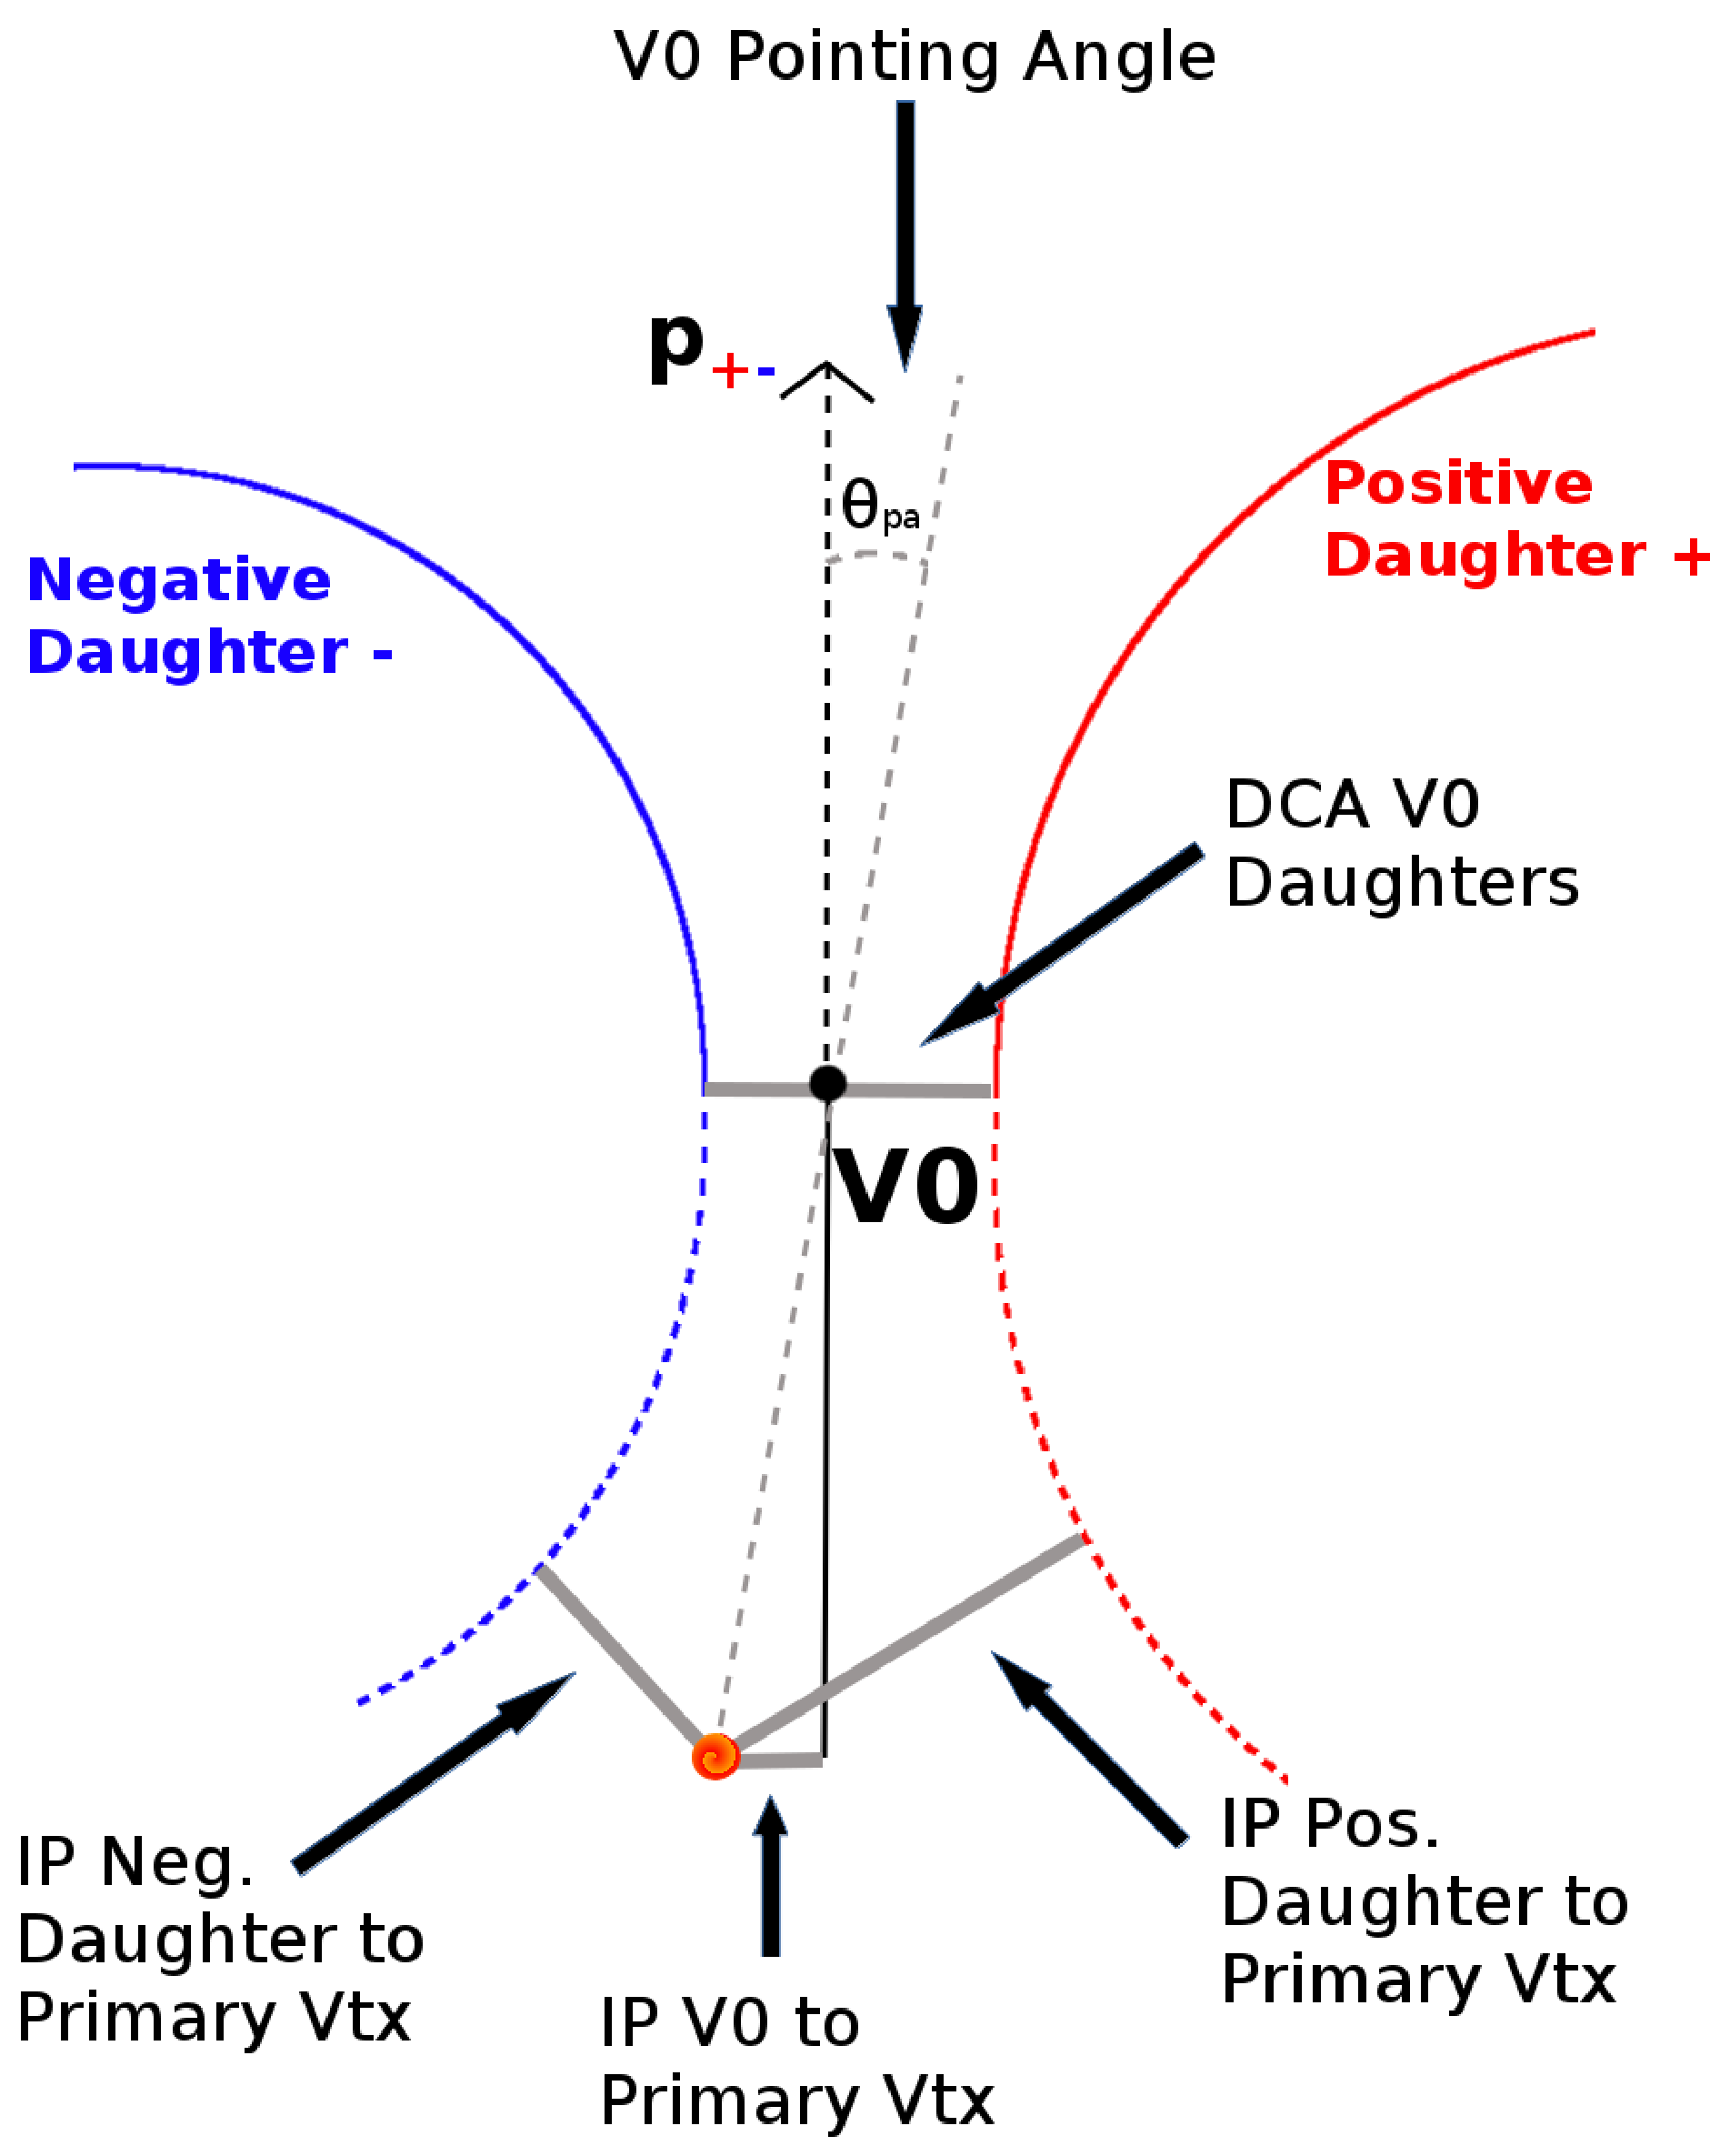
\includegraphics[width=0.9\linewidth]{3_DataSelection/Figures/V0CutsGeneral.pdf} 
  \caption[V0 Reconstruction]{V0 Reconstruction}
  \label{fig:V0Reconstruction}
\end{wrapfigure}
\end{comment}

\begin{figure}[h]
  \centering
  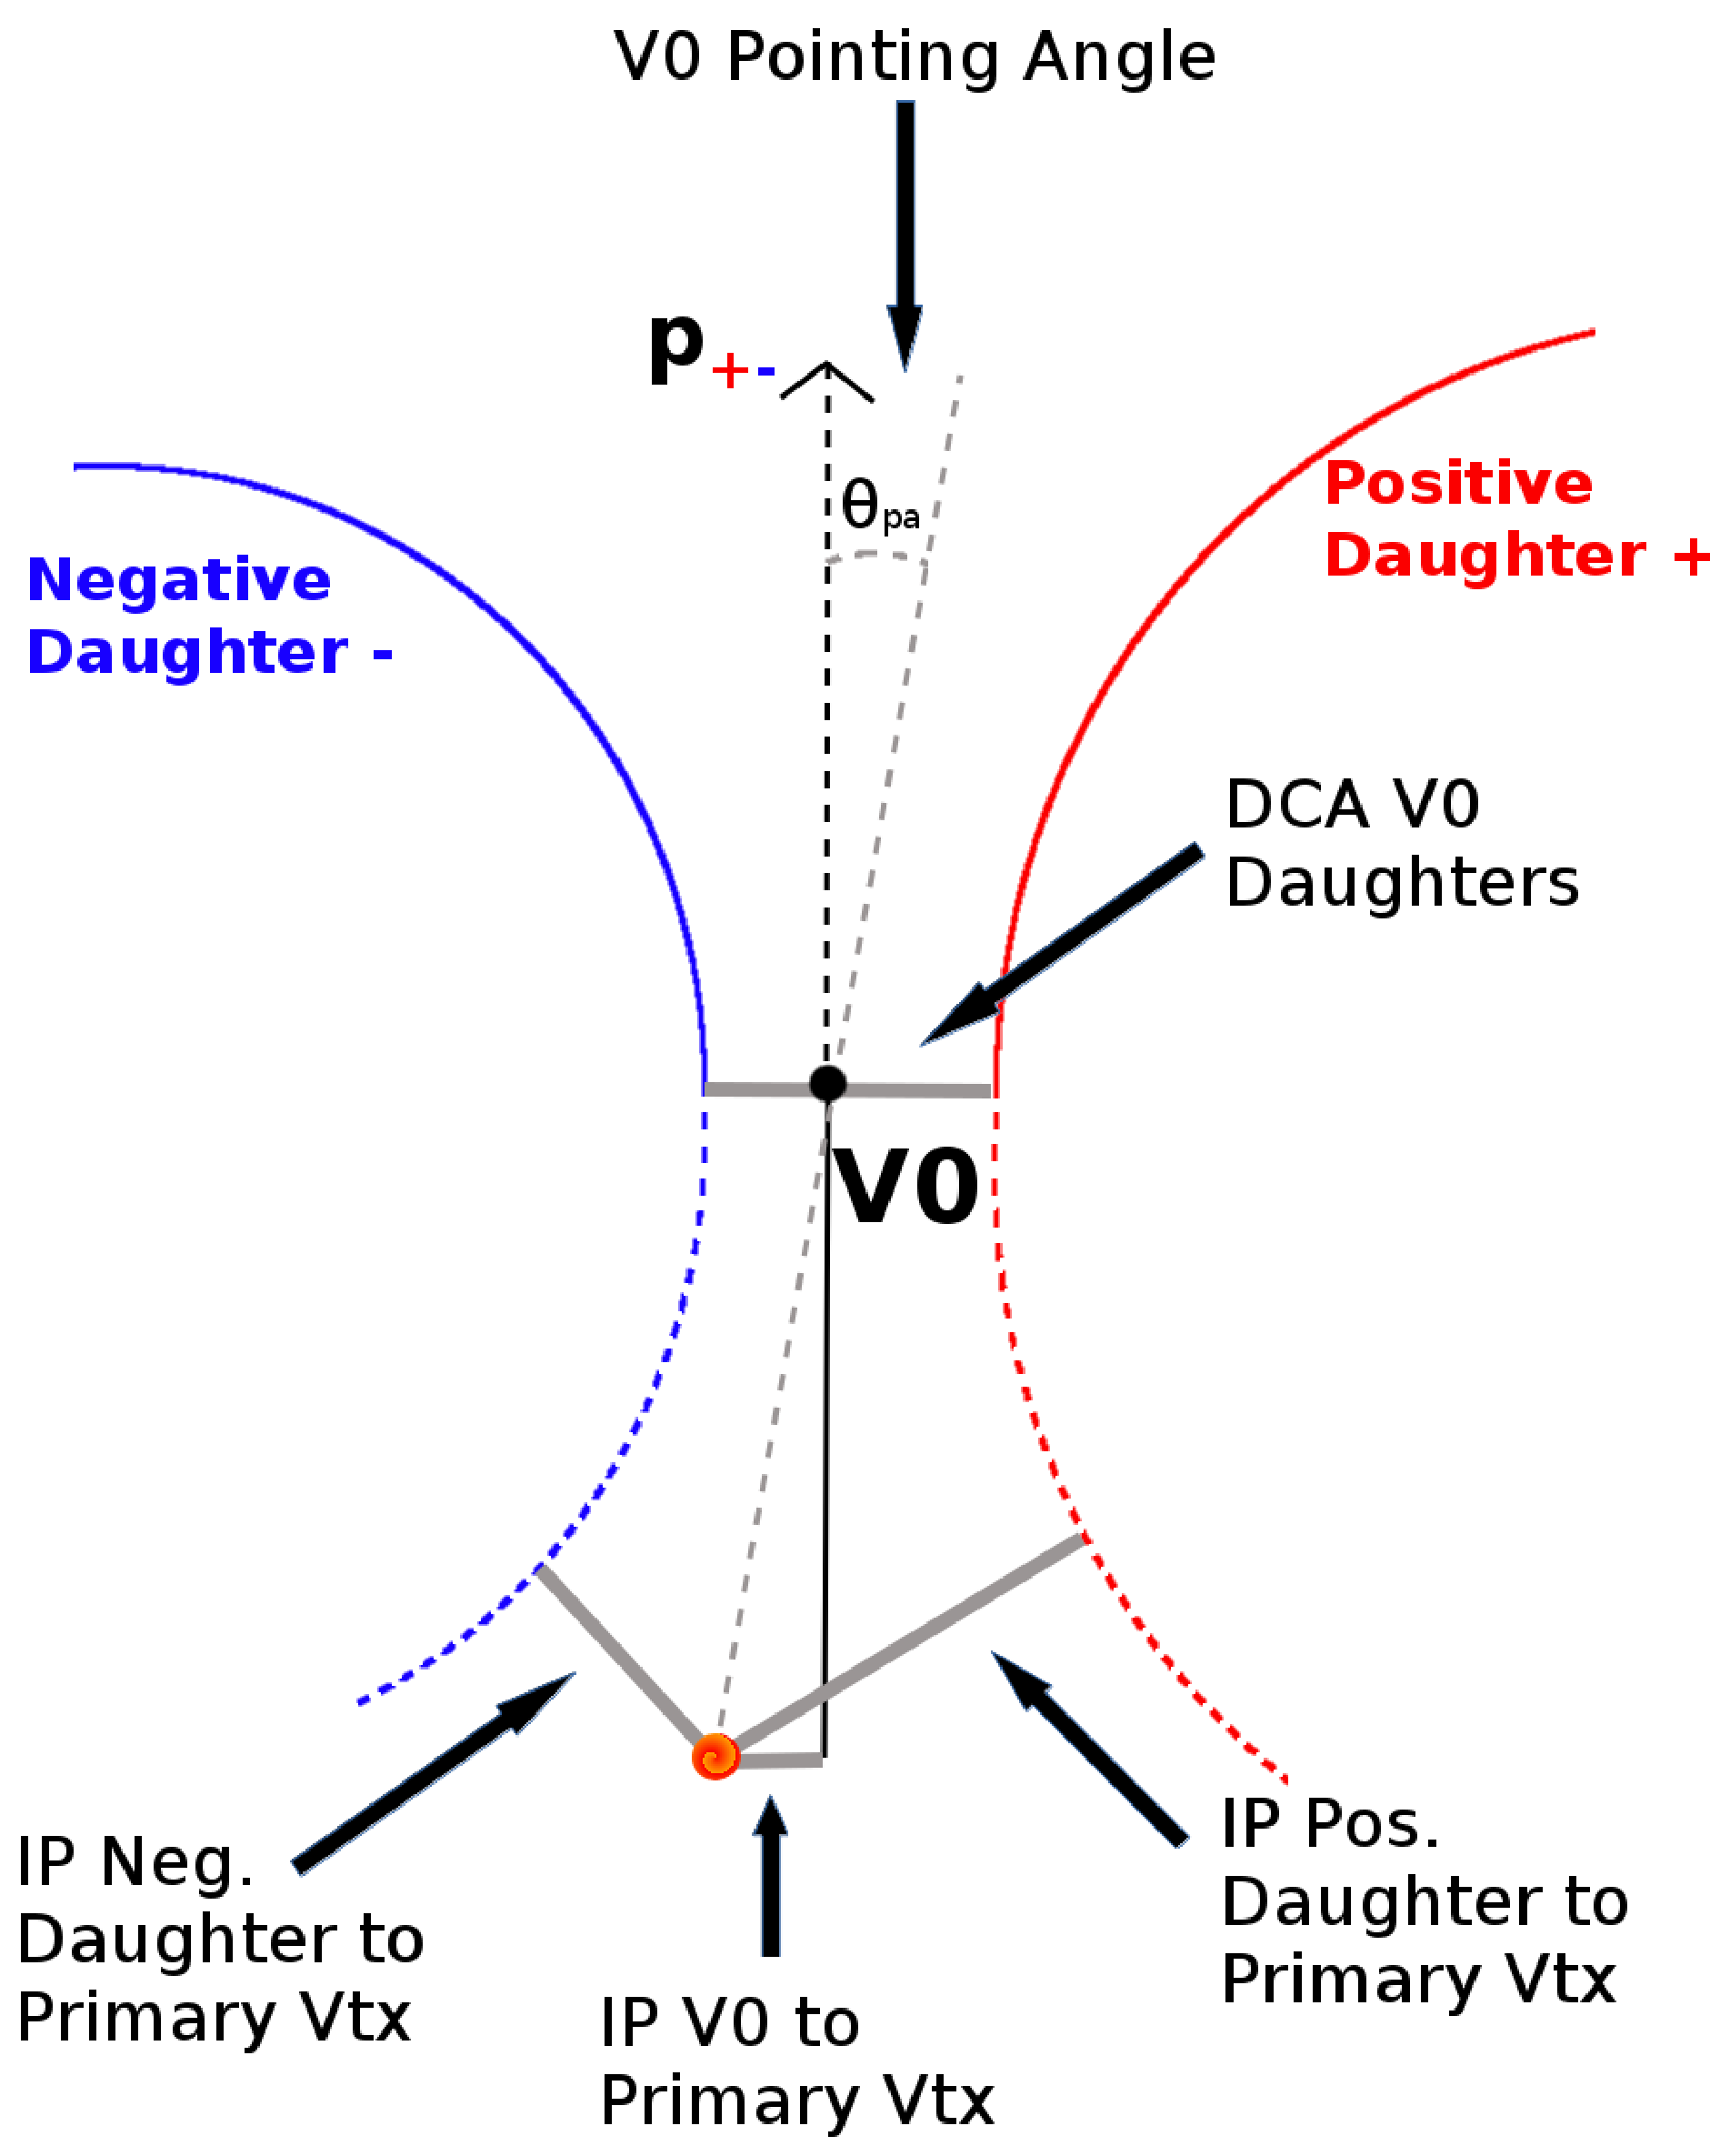
\includegraphics[width=0.5\textwidth]{3_DataSelection/Figures/V0CutsGeneral.pdf}
  \caption[V0 Reconstruction]{V0 Reconstruction}
  \label{fig:V0Reconstruction}
\end{figure}


In order to ensure a true and reliable signal, one must ensure good purity of the V0 collection.  The purity of the collection is calculated as:

\begin{equation}
 Purity = \frac{Signal}{Signal + Background}
\label{eqn:Purity}
\end{equation}

To obtain both the signal and background, the invariant mass distribution ($m_{\mathrm{inv}}$) of all V0 candidates must be constructed immediately before the final invariant mass cut.
Examples of such distributions can be found in Figures \ref{fig:cLamPurity} and \ref{fig:K0Purity}.
It is vital that the distribution be constructed immediately before the final $m_{\mathrm{inv}}$ cut, otherwise, it would be impossible to estimate the background.
As demonstrated in Figures \ref{fig:cLamPurity} and \ref{fig:K0Purity}, the background is fit with a polynomial outside of the peak region of interest in order to extrapolate an estimate for the background within the region.
Within the $m_{\mathrm{inv}}$ cut limits, the background is the region below the fit while the signal is the region above the fit.

\subfile{3_DataSelection/3.3_V0Selection/3.3.1_LambdaReconstruction.tex}
\subfile{3_DataSelection/3.3_V0Selection/3.3.2_K0sReconstruction.tex}
\subfile{3_DataSelection/3.3_V0Selection/3.3.3_V0PurityBgdEstimator.tex}

\end{document}
